\subchapter{Device Model - I2C device}{Objective: declare an I2C device
  and basic driver hooks called when this device is detected}

Throughout the upcoming labs, we will implement a driver for an I2C
device, which offers the functionality of an I2C nunchuk.

After this lab, you will be able to:

\begin{itemize}
\item Add an I2C device to a device tree
\item Implement basic \code{probe()} and \code{remove()} driver
functions and make sure that they are called when there is a
device/driver match.
\item Find your driver and device in \code{/sys}
\end{itemize}

\section{Setup}

Go to the \code{~/felabs/linux/src/linux} directory. Check out the
\code{3.13.y} branch. 

Now create a new \code{nunchuk} branch starting from the
\code{3.13.y} branch,  for your upcoming work on the nunchuk
driver.  

\section{Connecting the nunchuk}

Take the nunchuk device provided by your instructor.

We will connect it to the second I2C port of the CPU (\code{i2c1}),
which pins are available on the \code{P9} connector.

Download a useful document sharing useful details about the nunchuk
and its connector: 
\url{http://web.engr.oregonstate.edu/~sullivae/ece375/pdf/nunchuk.pdf}

Now we can identify the 4 pins of the nunchuk connector:

\begin{center}
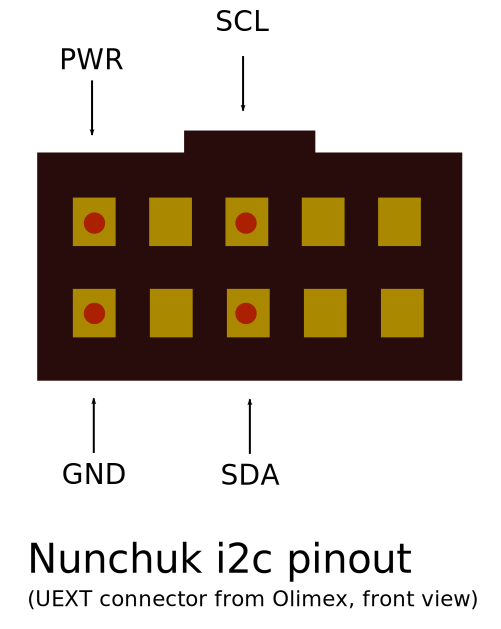
\includegraphics[width=4cm]{labs/kernel-i2c-device-model/nunchuk-pinout.pdf}
\end{center}

Open the System Reference Manual that you downloaded earlier,
and look for "connector P9" in the table of contents, and then
follow the link to the corresponding section. Look at the table listing
the pinout of the P9 connector.

Now connect the nunchuk pins:
\begin{itemize}
\item The \code{GND} pin to P9 pins 1 or 2 (\code{GND})
\item The \code{PWR} pin to P9 pins 3 or 4 (\code{DC_3.3V})
\item The \code{CLK} pin to P9 pin 17 (\code{I2C1_SCL})
\item The \code{DATA} pin to P9 pin 18 (\code{I2C1_SDA})
\end{itemize}

\begin{center}
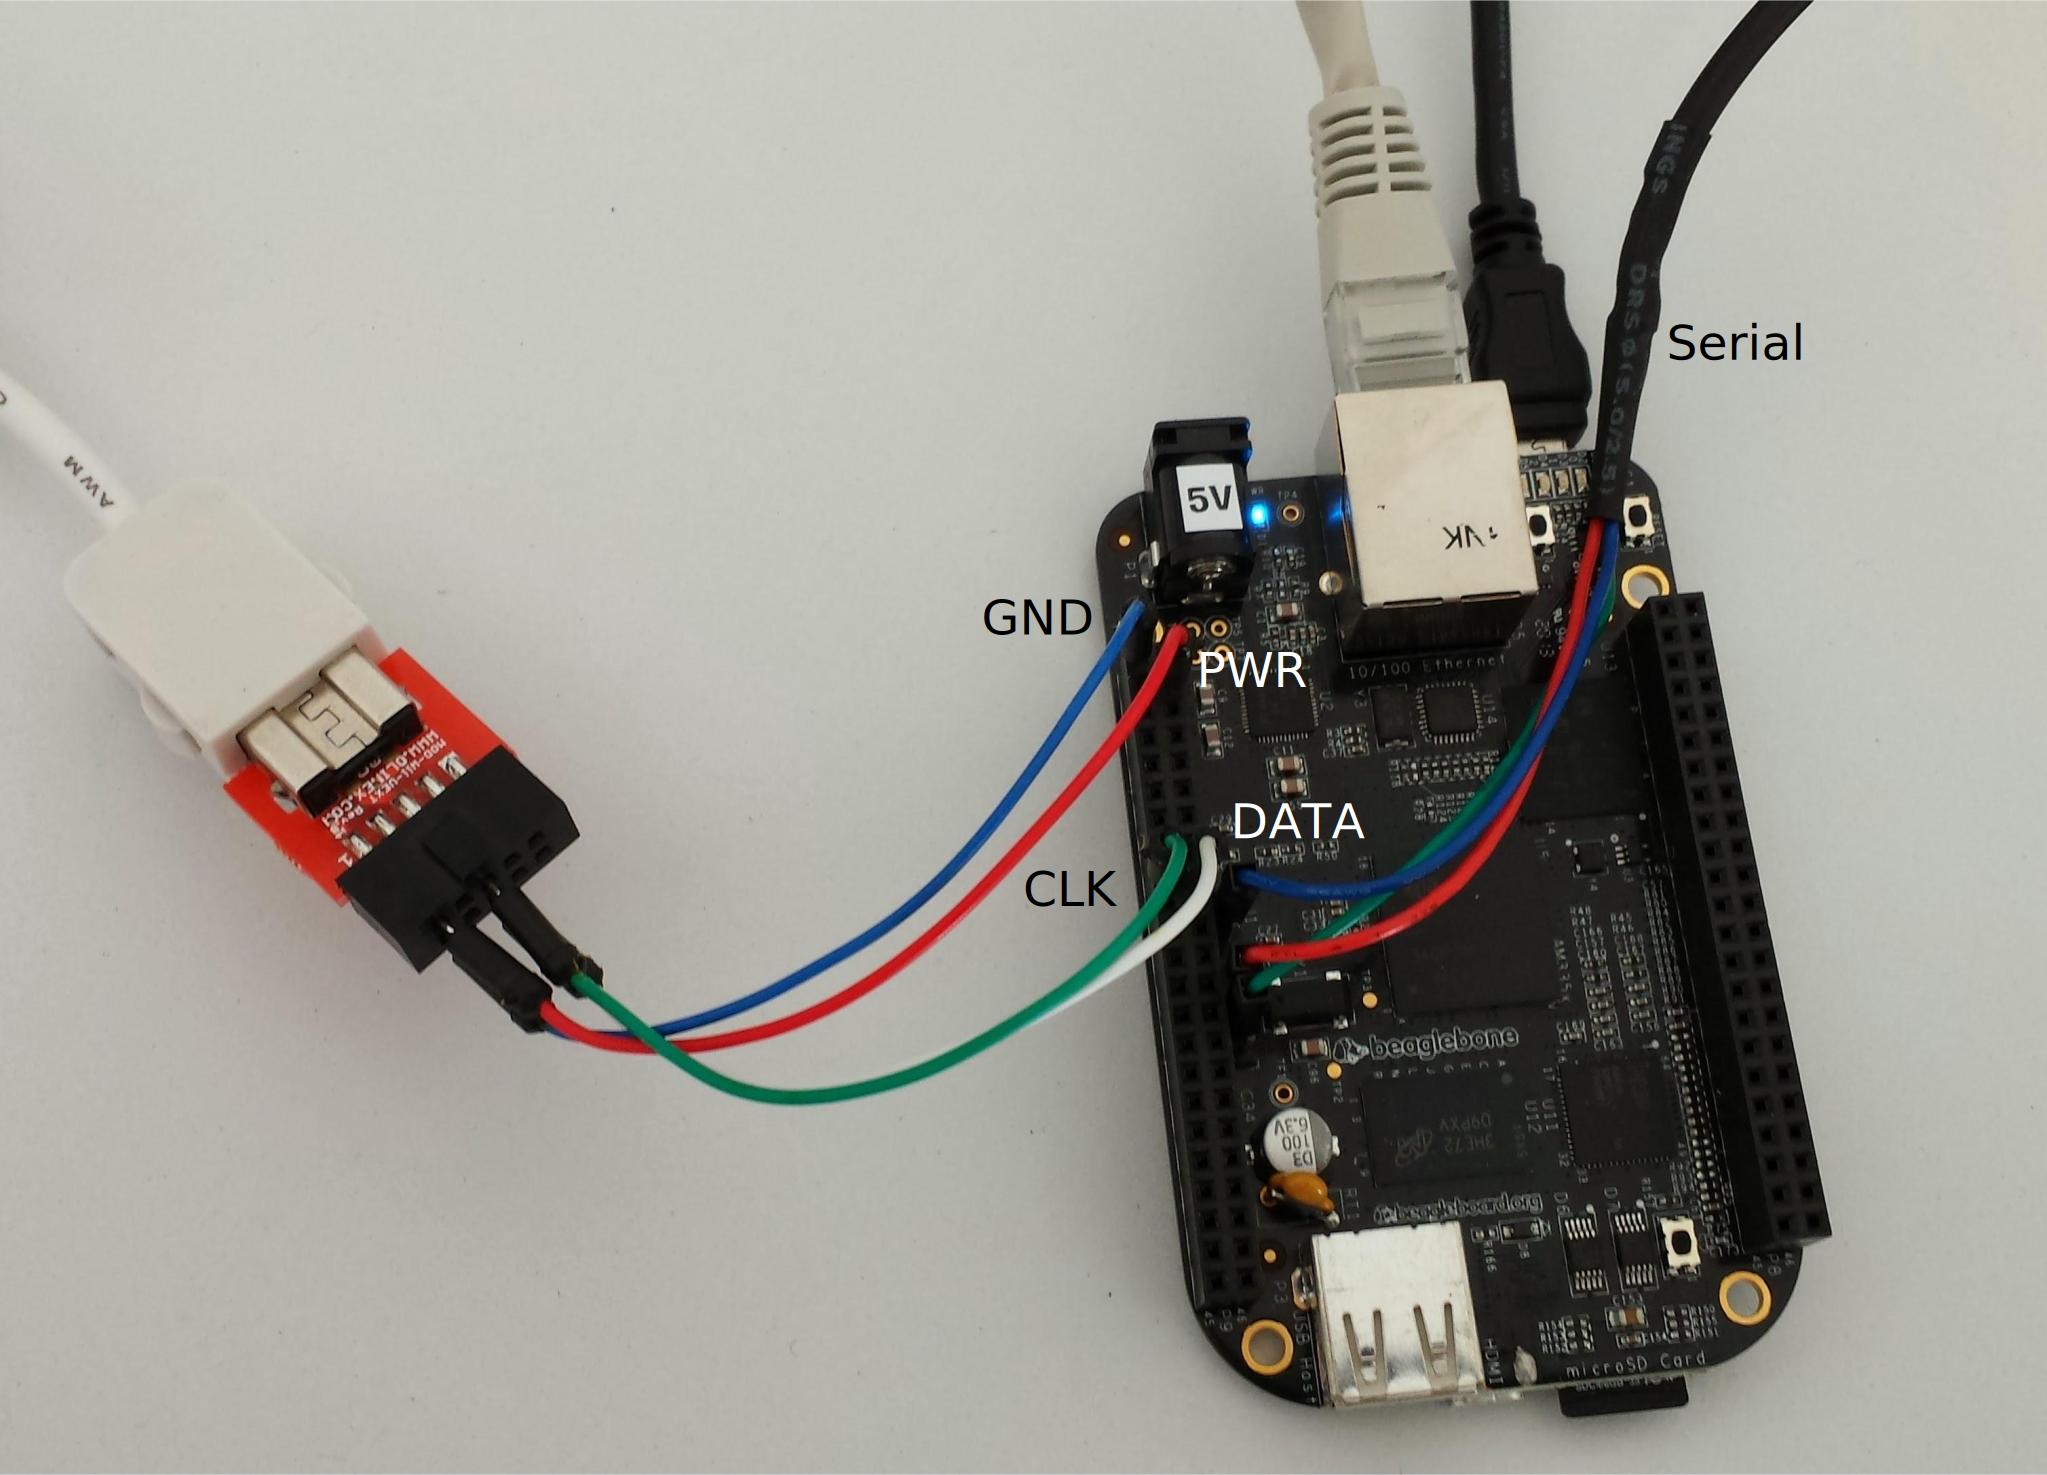
\includegraphics[width=12cm]{labs/kernel-i2c-device-model/bbb-connect-nunchuk.pdf}
\end{center}

\section{Update the board device tree}

To let the Linux kernel handle a new device, the first thing is to add a
description for it in the board device tree.

We will have to do two things:

\begin{enumerate}
\item Add a node declaring a second I2C bus (\code{i2c1}) 
\item Add a child node to this bus, corresponding to the Nunchuk device. 
\end{enumerate}

\subsection{Declare a second I2C bus}

First, find in which DTS file the first I2C bus (\code{i2c0}) for the 
BeagleBone Black is instantiated and in which file it is defined.

Find the definitions for \code{i2c1}. What is the base address of its
registers? Also find the same address in the processor datasheet
\footnote{Tip: to do your search, put an underscore character in the middle
of the address, as in \code{FFFF_FFFF}... that's how addresses are written in the
TI datasheet).}.

Then, imitating the definitions found for \code{i2c0},
modify the \code{arch/arm/boot/dts/am335x-boneblack.dts}
file to instantiate \code{i2c1}, functioning at 100 KHz.

\subsection{Declare the Nunchuk device} 

As a child node to this second bus, declare the \code{nunchuk}
device, choosing \code{nintendo,nunchuk} for its \code{compatible}
property. You will find the I2C slave address of the nunchuk on the
nunckuk document that we have used earlier \footnote{This I2C slave
addressed is enforced by the device itself. You can't change it.}.

\subsection{Checking the device tree on the running system}

Now that you have modified the board device tree, recompile your
DTB and copy the updated version to the tftp server home directory.

Boot the board.

Through the \code{/proc/device-tree} directory, it is possible to check
the Device Tree settings that your system has loaded. That's useful when
you are not sure exactly which settings were actually loaded. 

For example, you can check the presence of a new \code{nunchuk} node in
your device tree:

\begin{verbatim}
# find /proc/device-tree -name "*nunchuk*"
/proc/device-tree/ocp/i2c@4802a000/nunchuk@52
\end{verbatim}

Using the Device Tree Compiler (\code{dtc}, which we put in the root
filesystem), you can also check the whole Device Tree structure. That's
better than checking the source files and includes in the source
directory!

\begin{verbatim}
# dtc -I fs /proc/device-tree/
\end{verbatim}

Look for \code{i2c1} and \code{nunchuk} in the output of this command,
and see where the nodes are instantiated. Don't hesitate to ask your
instructor for questions!

\section{Implement a basic I2C driver for the nunchuk}

It is now time to start writing the first building blocks of the I2C
driver for our nunchuk.

In a new terminal, go to
\code{~/felabs/linux/modules/nfsroot/root/nunchuk/}.  This directory
contains a Makefile and an almost empty \code{nunchuk.c} file.

Now, you can compile your out-of-tree module by running \code{make}. As
the current directory is part of the NFS root that the board boots on,
the generated \code{.ko} file will immediately be visible on the board
too.

Relying on explanations given during the lectures, fill the
\code{nunchuk.c} file to implement:

\begin{itemize}
\item \code{probe()} and \code{remove()} functions that will
      be called when a nunchuk is found.
      For the moment, just put a call to \code{pr_info()} inside
      to confirm that these function are called.
\item Initialize an \code{i2c_driver} structure, and register
      the i2c driver using it. Make sure that you use
      a \code{compatible} property that matches the one in the
      Device Tree.
\end{itemize}

You can now compile your module and reboot your board, to 
boot with the updated DTB.

\section{Driver tests}

You can now load the \code{/root/nunchuk/nunchuk.ko} file.
You need to check that the \code{probe()} function gets called
then, and that the \code{remove()} function gets called too
when you remove the module.

Once your new Device Tree and module work as expected, commit
your DT changes in your Linux tree:

\begin{verbatim}
git commit -sa 
\end{verbatim}

\section{Exploring /sys}

Take a little time to explore \code{/sys}:

\begin{itemize}
\item Find the representation of your driver. That's a way
      of finding the matching devices.
\item Find the representation of your device, containing its name.
      You will find a link to the driver too.
\end{itemize}
